\documentclass[UTF8]{ctexart}
\usepackage{amsmath}
\usepackage{forest}
\usepackage{algorithm}
\usepackage{algorithmic}
\usepackage{graphicx}
\usepackage{tabularx}
\title{\vspace{-4cm}2023数据库概论第二次作业}
\author{2000013058 杨仕博}
\date{\today}
\begin{document}
\maketitle

\subsection{}

聚集:

记录若干棋手参加过的比赛和在每场比赛中最常使用的开局。

这里,实体是棋手、比赛和开局。棋手-参加-比赛被聚集成另一个
实体,这个实体和开局的关系是最常使用。

优点:此时“参加”的联系与“最常使用”的联系存在重叠,“聚集”可以
抽象这种联系,清楚地刻画“参加”这种联系与“开局”之间的“最常使用”
联系。

弱实体:

记录一场拍卖会中,每场拍卖活动的成交价和三次未成交的最高报价
的金额。

这里,每场“拍卖活动”是实体,具有“成交价”属性,由拍卖场次标识,
而每个“未成交的高报价”由它所在的拍卖活动和它的出价排名确定,
具有“金额”属性,在ER图中以弱实体的形式呈现。“成交价”和
“拍卖活动”有“隶属”关系。

优点:

解决了“未成交的高报价”只能通过“拍卖活动”标识,没有“主码”不能
作为“实体”存在的问题,避免了属性的冗余,并且能够使“未成交的高报价”
像实体一样得到足够清晰的刻画。

细化/泛化:

我们希望记录某社会中人的财产情况,其中高收入群体的公益活动
付出情况与其中低收入群体接受社会福利的情况。

这里,社会中的人为实体,他们拥有“财产情况”属性,这个属性
的记录与“人”之间不同的群体无关,是所有人都具备的属性,
因而适应于“泛化”结构;“高收入群体”
和“低收入群体”是“社会中的人”的子集,而且他们的属性也需要记录,
因而适应于“细化”结构。

优点:“社会中的人”是总体,他的“财产情况”属性是无论什么类别
的人都有的属性,“泛化”可以将所有类别的人合成一个整体记录该
属性,不用在每个特定群组中再分别记录。
“高收入群体”和“低收入群体”分别有区别于其他实体的
“公益活动付出”与“接受社会福利”的属性,“细化”可以根据
这一点在已经刻画了整体的财产情况的条件下进一步精确地刻画出
其中的“高收入群体”和“低收入群体”,并更精确地刻画他们的属性。

\subsection{}

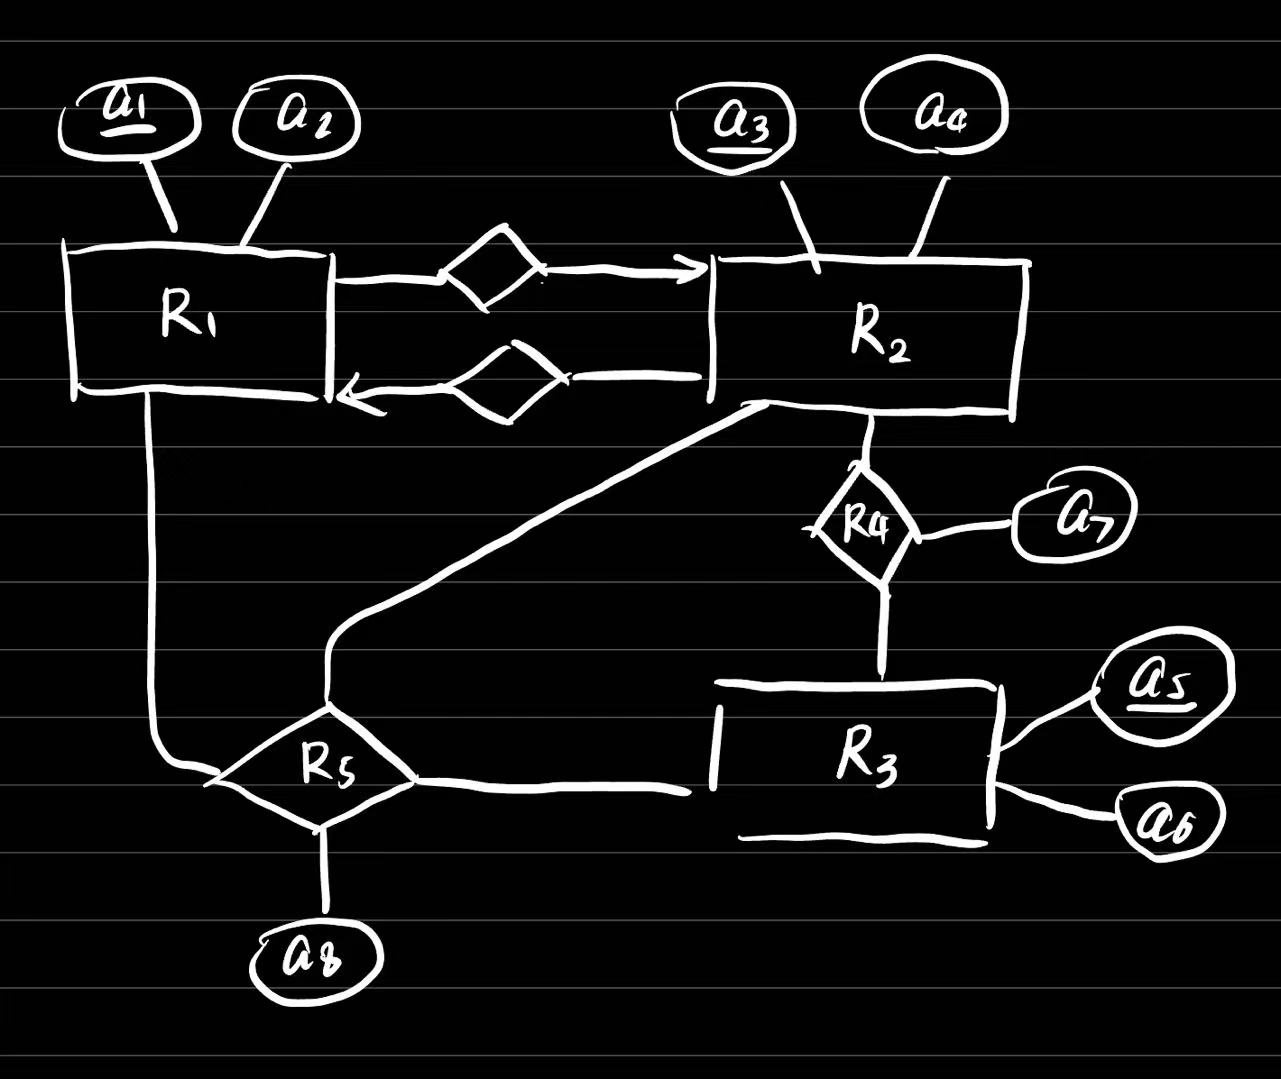
\includegraphics[width=\textwidth]{./pics/2.jpeg}

\subsection{}

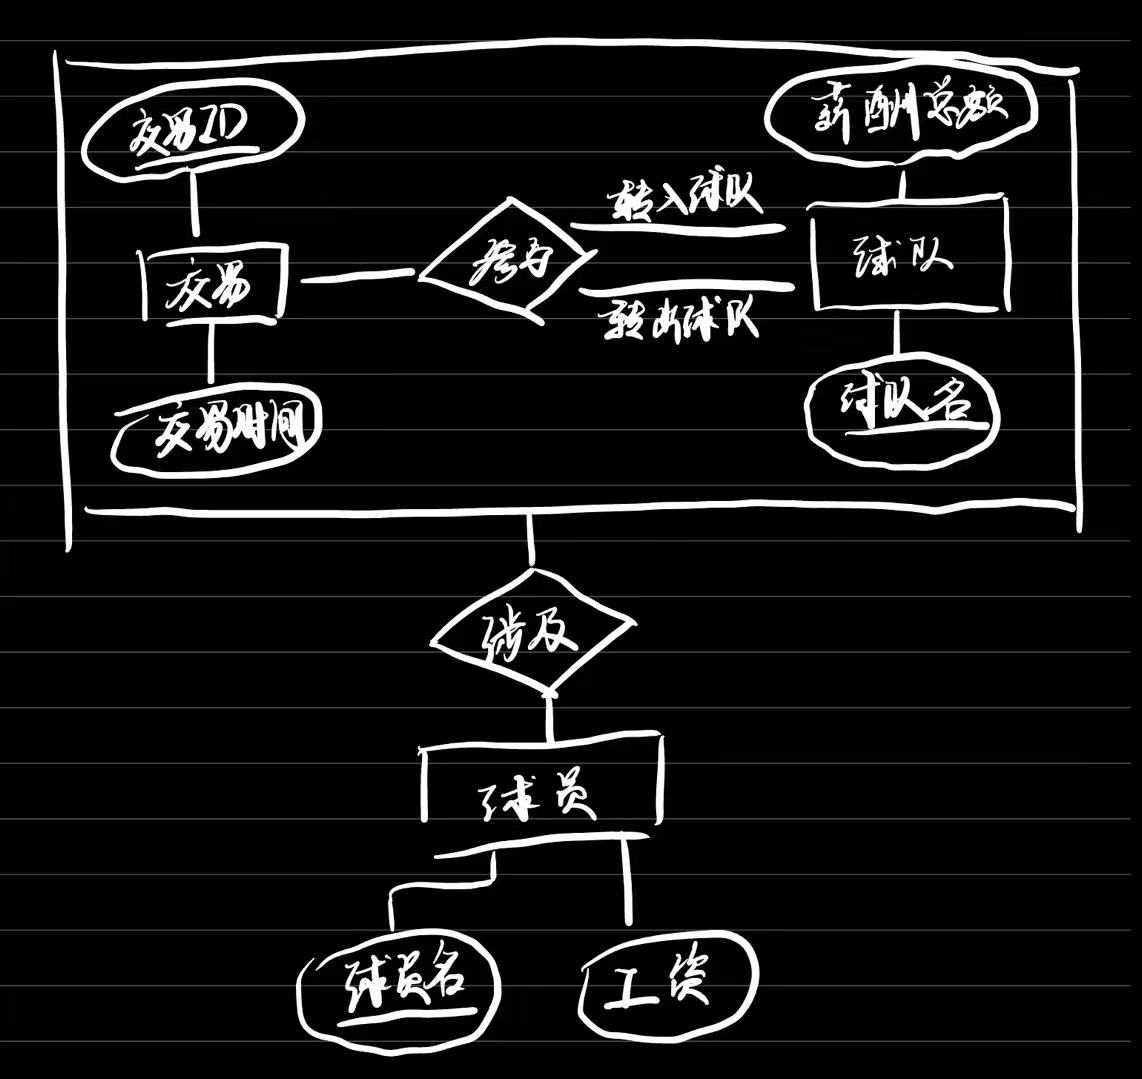
\includegraphics[width=\textwidth]{./pics/3.jpeg}

\subsection{}

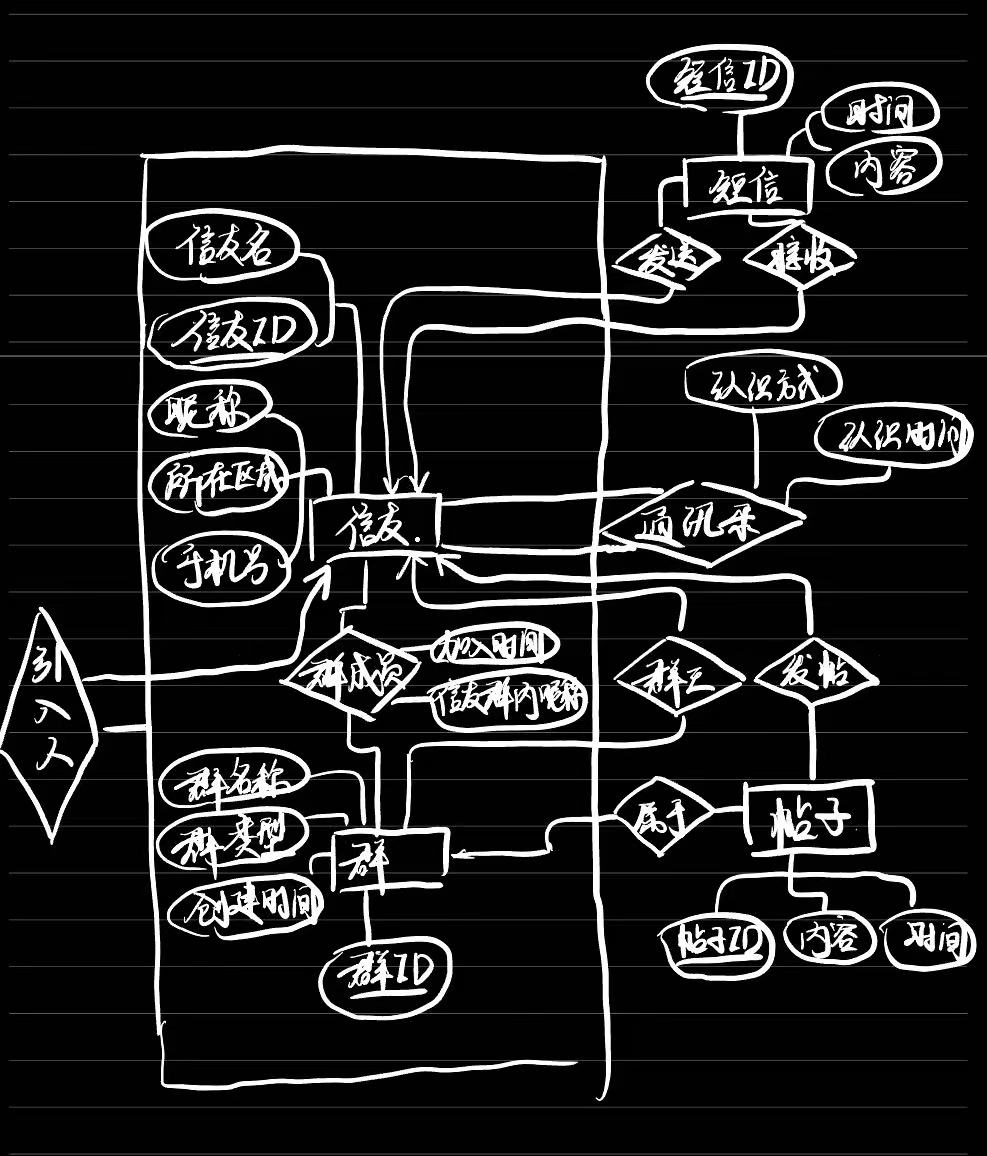
\includegraphics[width=\textwidth]{./pics/4.jpeg}

\subsection{}

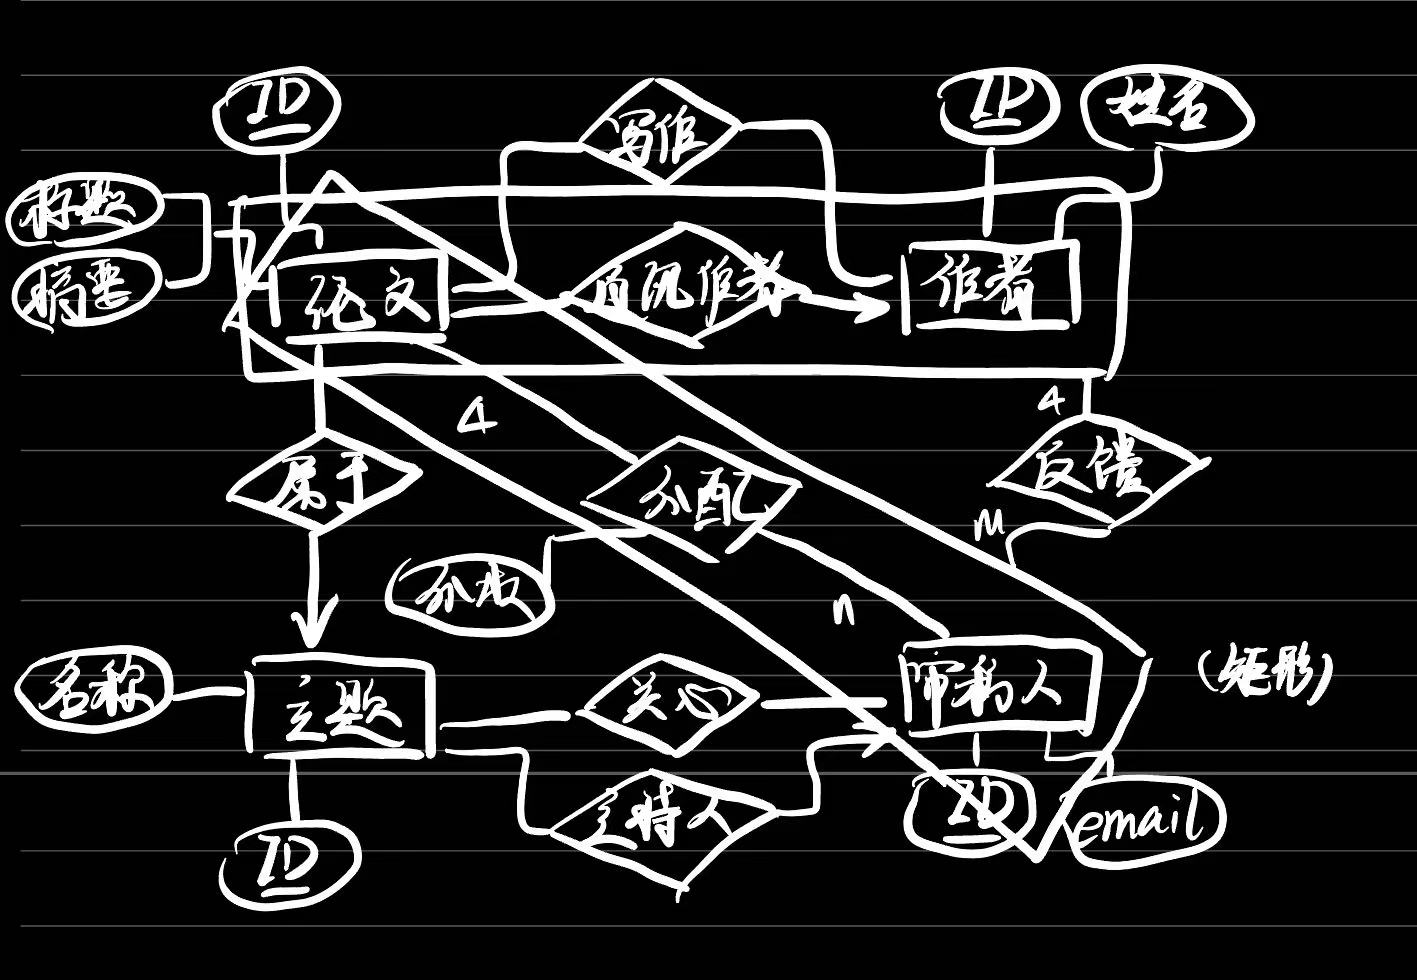
\includegraphics[width=\textwidth]{./pics/5.jpeg}

\subsection{}

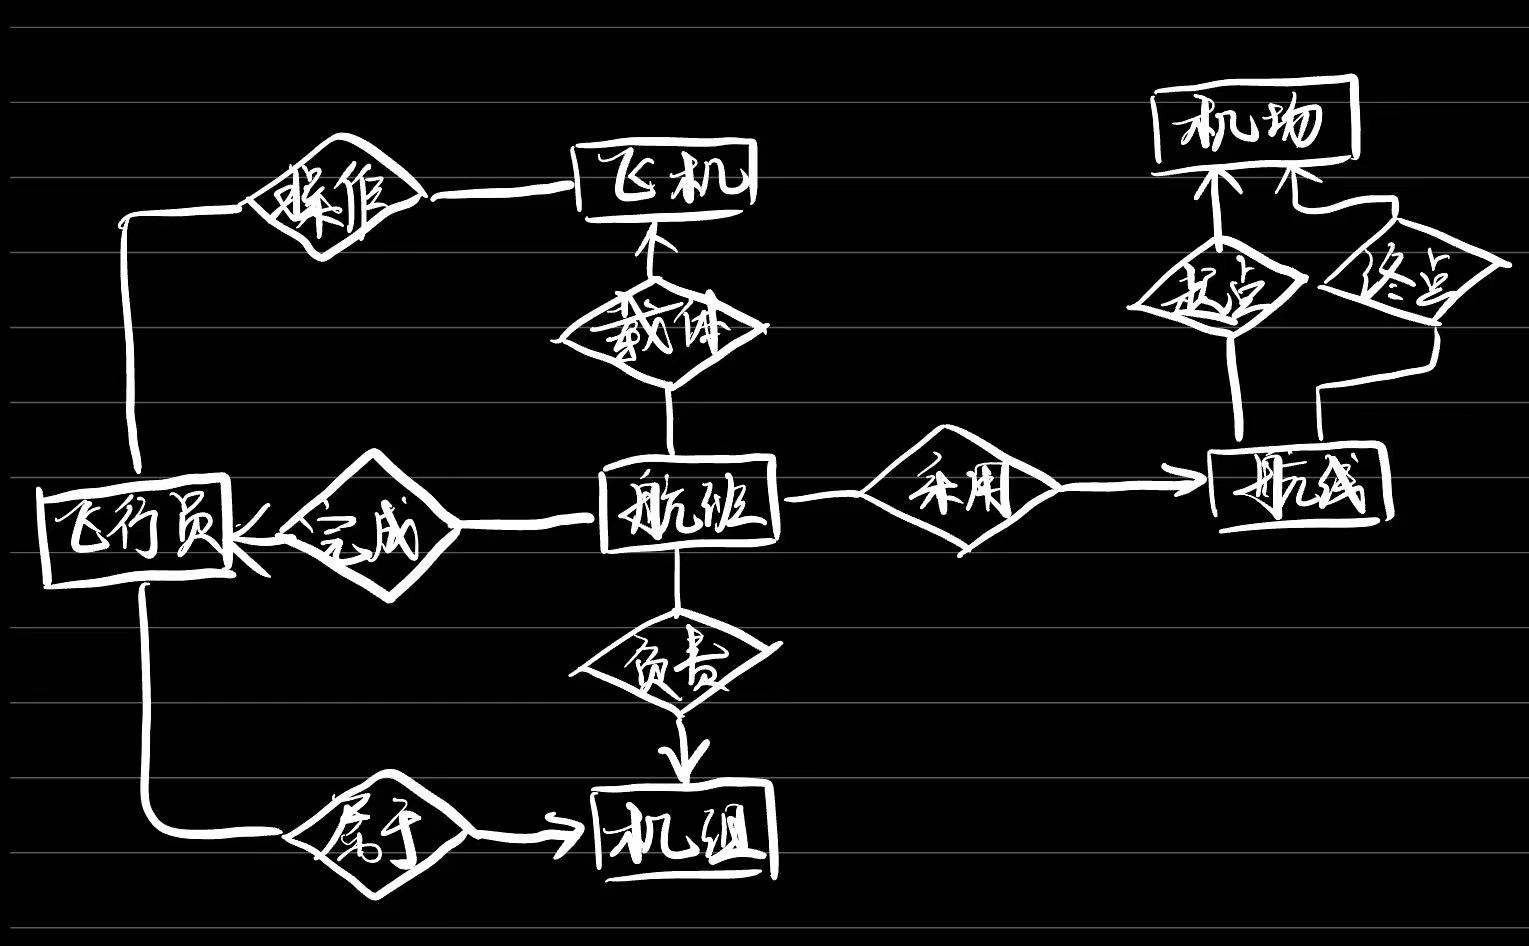
\includegraphics[width=\textwidth]{./pics/6.jpeg}

\end{document}